\chapter{Manual de Usuario}
\label{chap:manual}
Para acceder a la herramienta se accederá a través de una navegador web a la dirección \url{https://mementoparking.herokuapp.com/}, donde podremos observar la página de inicio (ver figura \ref{fig:home}). Para darnos de alta en el sistema podremos pulsar en el botón \textit{regístrate} que aparece en el centro de la página o mediante el enlace que aparece en la esquina superior derecha de la pantalla.

	\begin{figure}[h!]
		\centering
		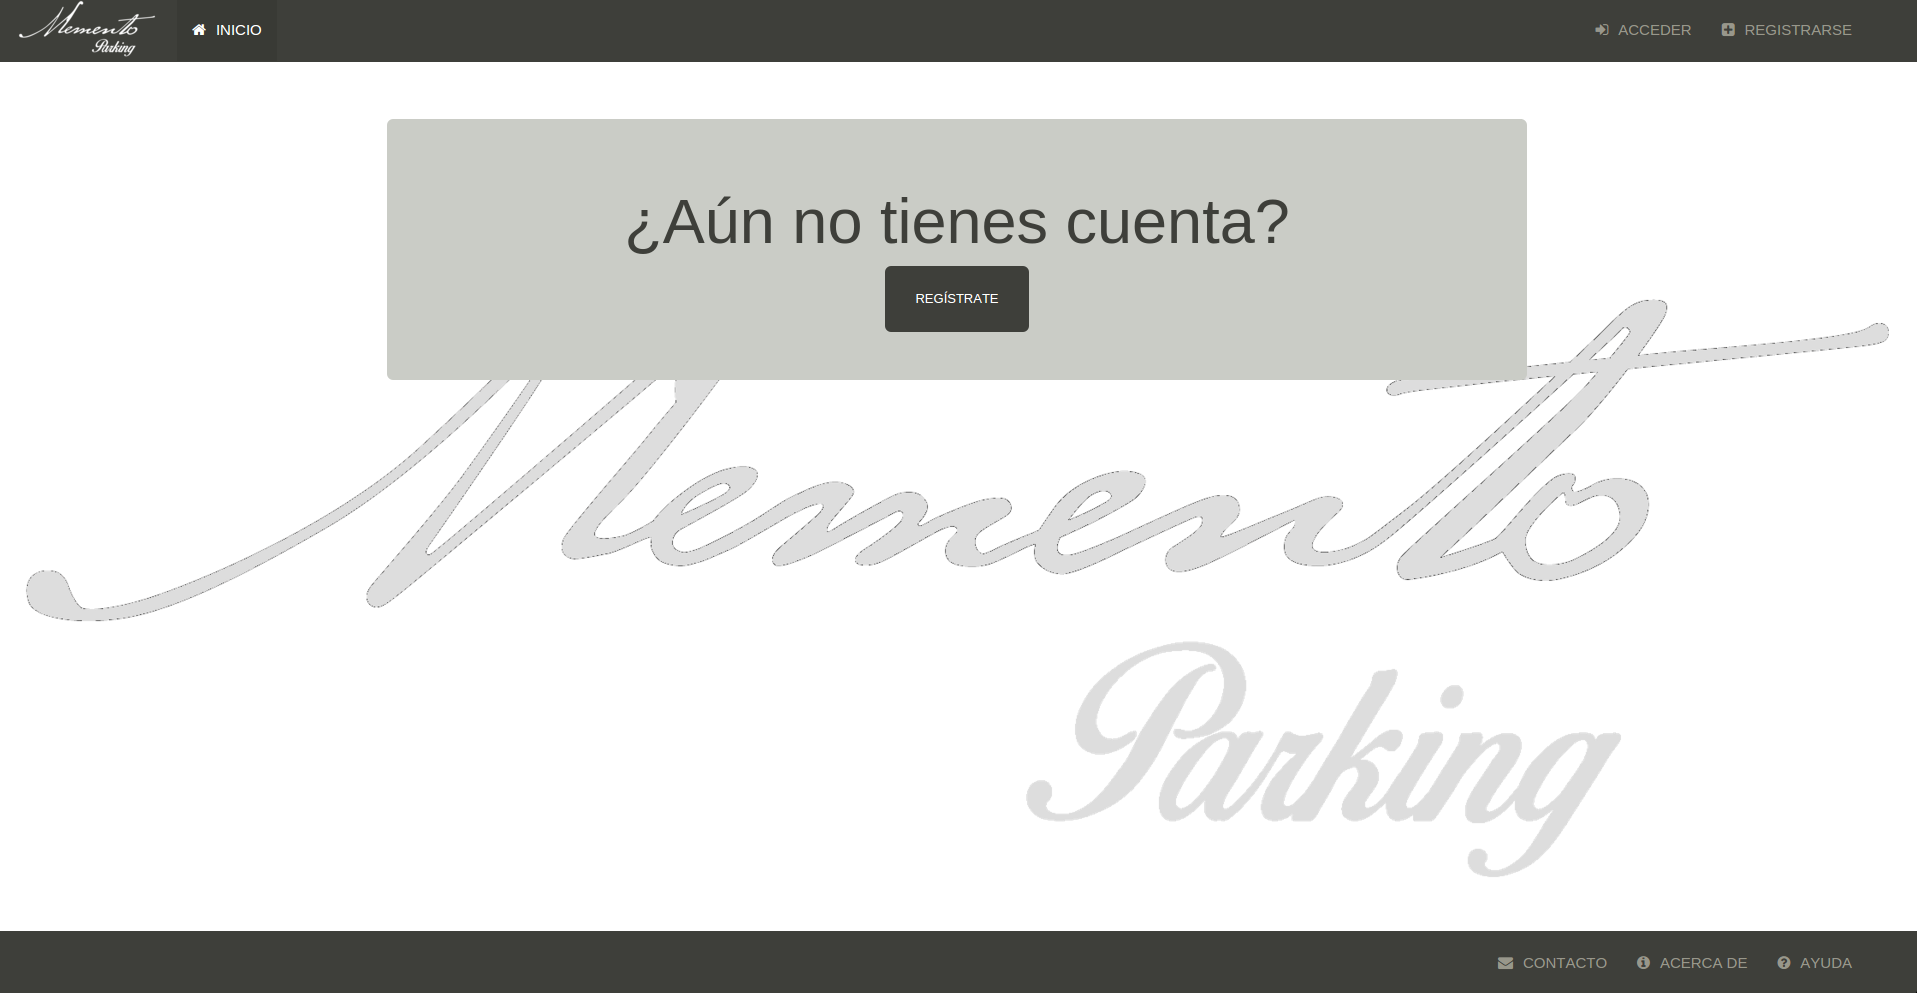
\includegraphics[width=15cm, fbox={\fboxrule} 4mm]{images/06-manual/01-home.png}
		\caption{Página principal}
		\label{fig:home}
	\end{figure}

Una vez accedido a la página de registro (ver figura\ref{fig:register}) podemos observar los campos a rellenar para darnos de alta como nuevo usuario.

	\begin{figure}[h!]
		\centering
		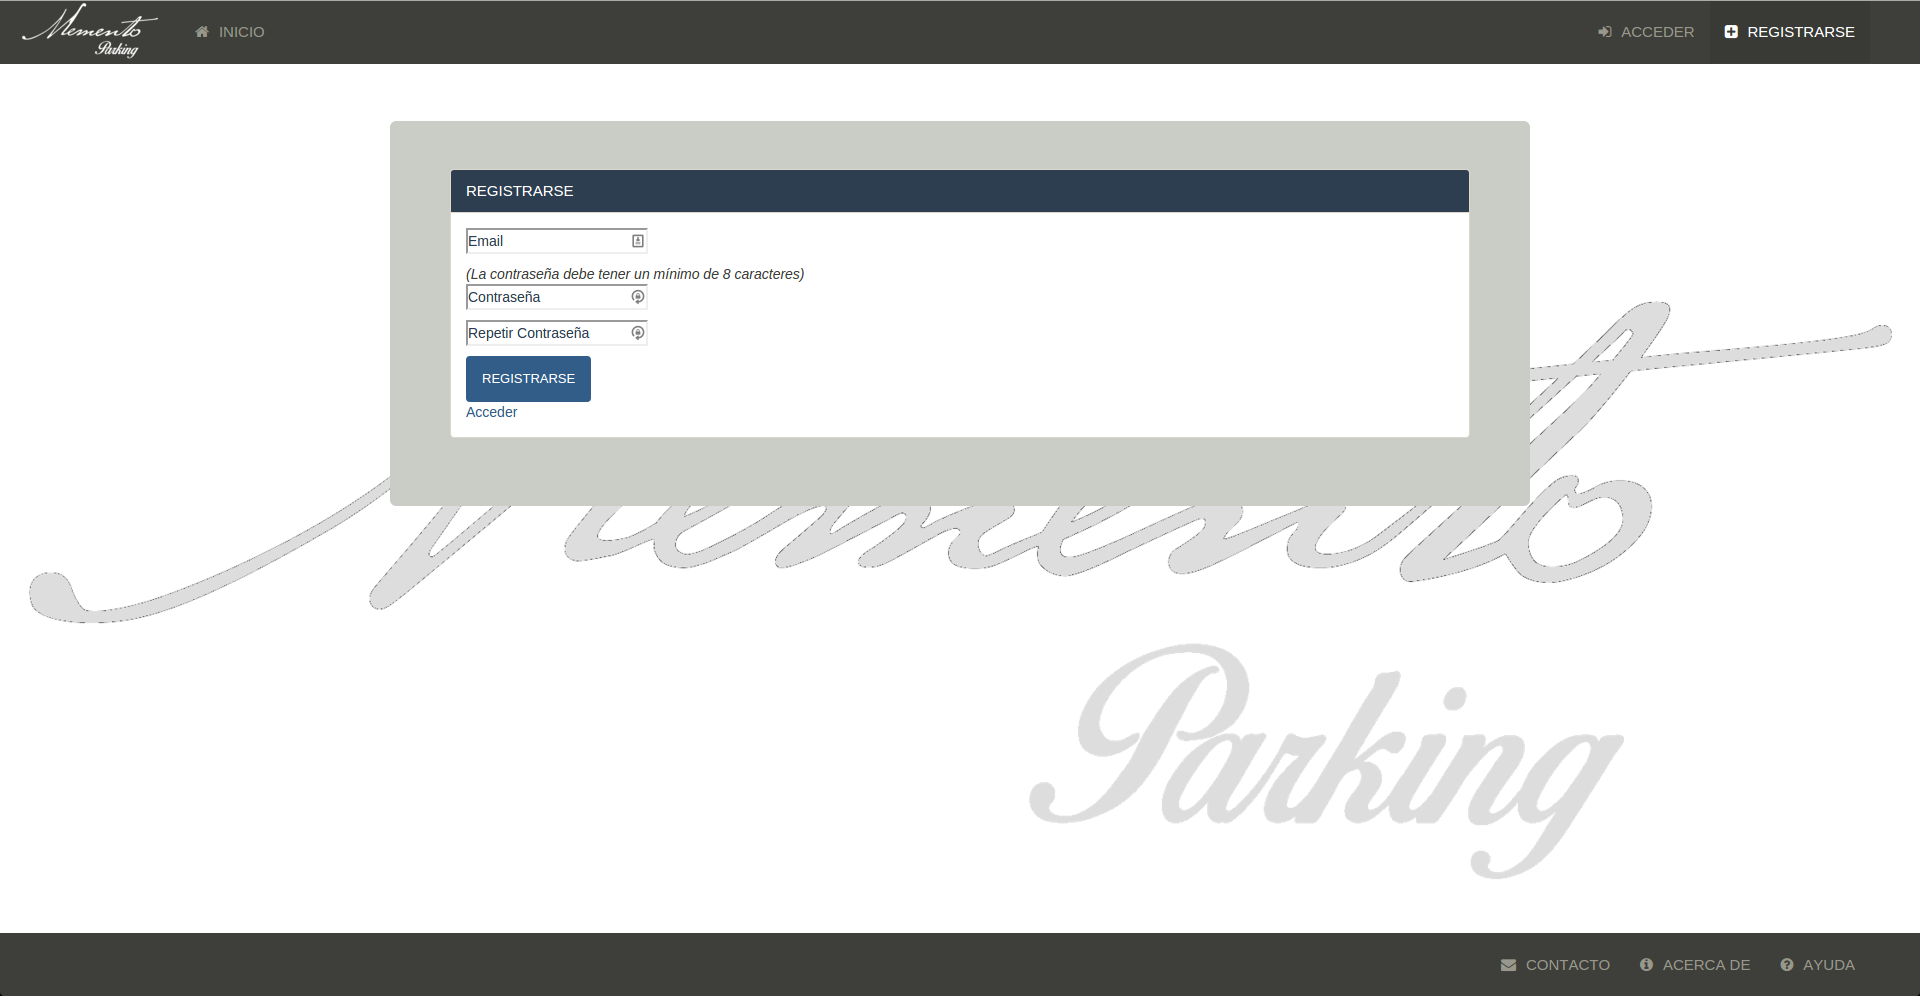
\includegraphics[width=15cm, fbox={\fboxrule} 4mm]{images/06-manual/02-register.png}
		\caption{Página registro}
		\label{fig:register}
	\end{figure}
	
Una vez dado de alta como nuevo usuario, yendo a la página de acceso e introduciendo nuestro email y contraseña (ver figura \ref{fig:sign_in})podremos entrar a las páginas reservadas a los usuarios registrados. Una vez nos hemos autenticado en el sistema correctamente, volveremos al página de inicio, donde podremos observar un mensaje informándonos de que hemos accedido correctamente y también que la barra de navegación ha cambiado su aspecto, dándonos la bienvenida y mostrando un menú bien con nuestro nombre en el caso de que hayamos editado nuestros datos o bien con el correo electrónico que hemos utilizado para acceder al sistema (ver figura \ref{fig:home_sign_in}).

	\begin{figure}[h!]
		\centering
		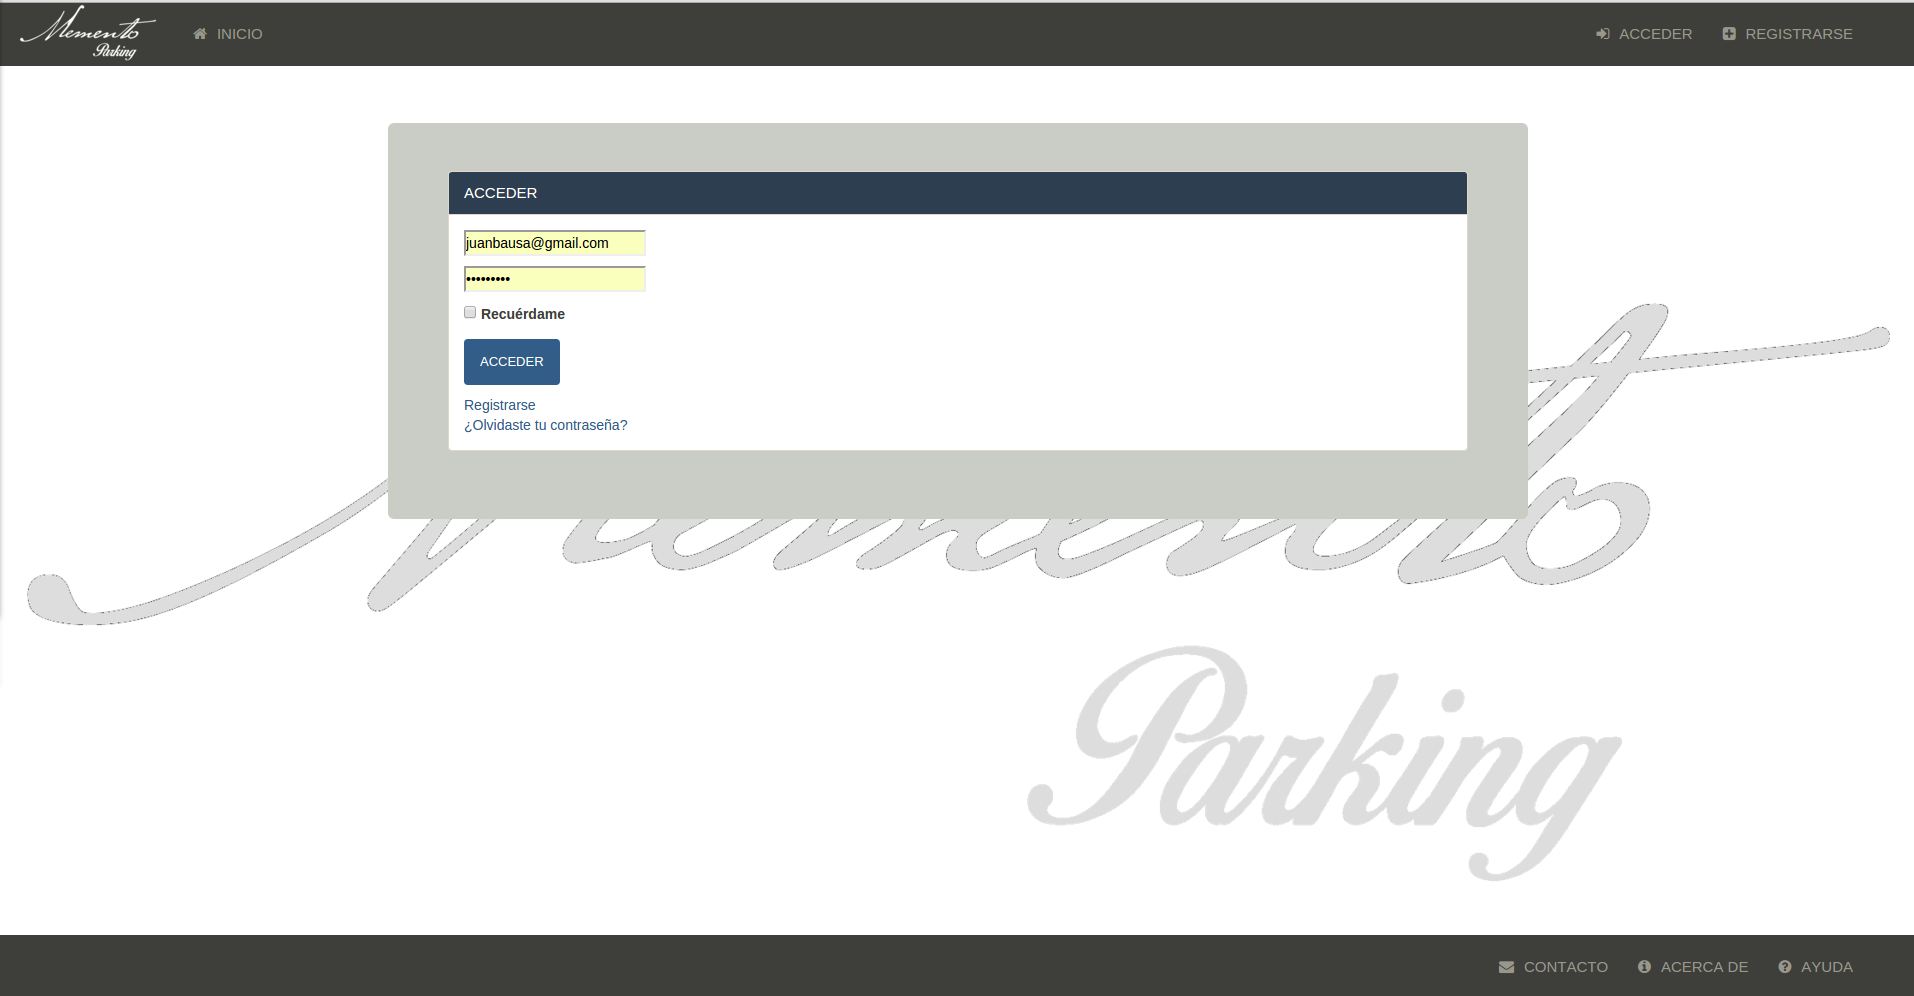
\includegraphics[width=15cm, fbox={\fboxrule} 4mm]{images/06-manual/03-sign_in.png}
		\caption{Página acceso}
		\label{fig:sign_in}
	\end{figure}
	
	\begin{figure}[h!]
		\centering
		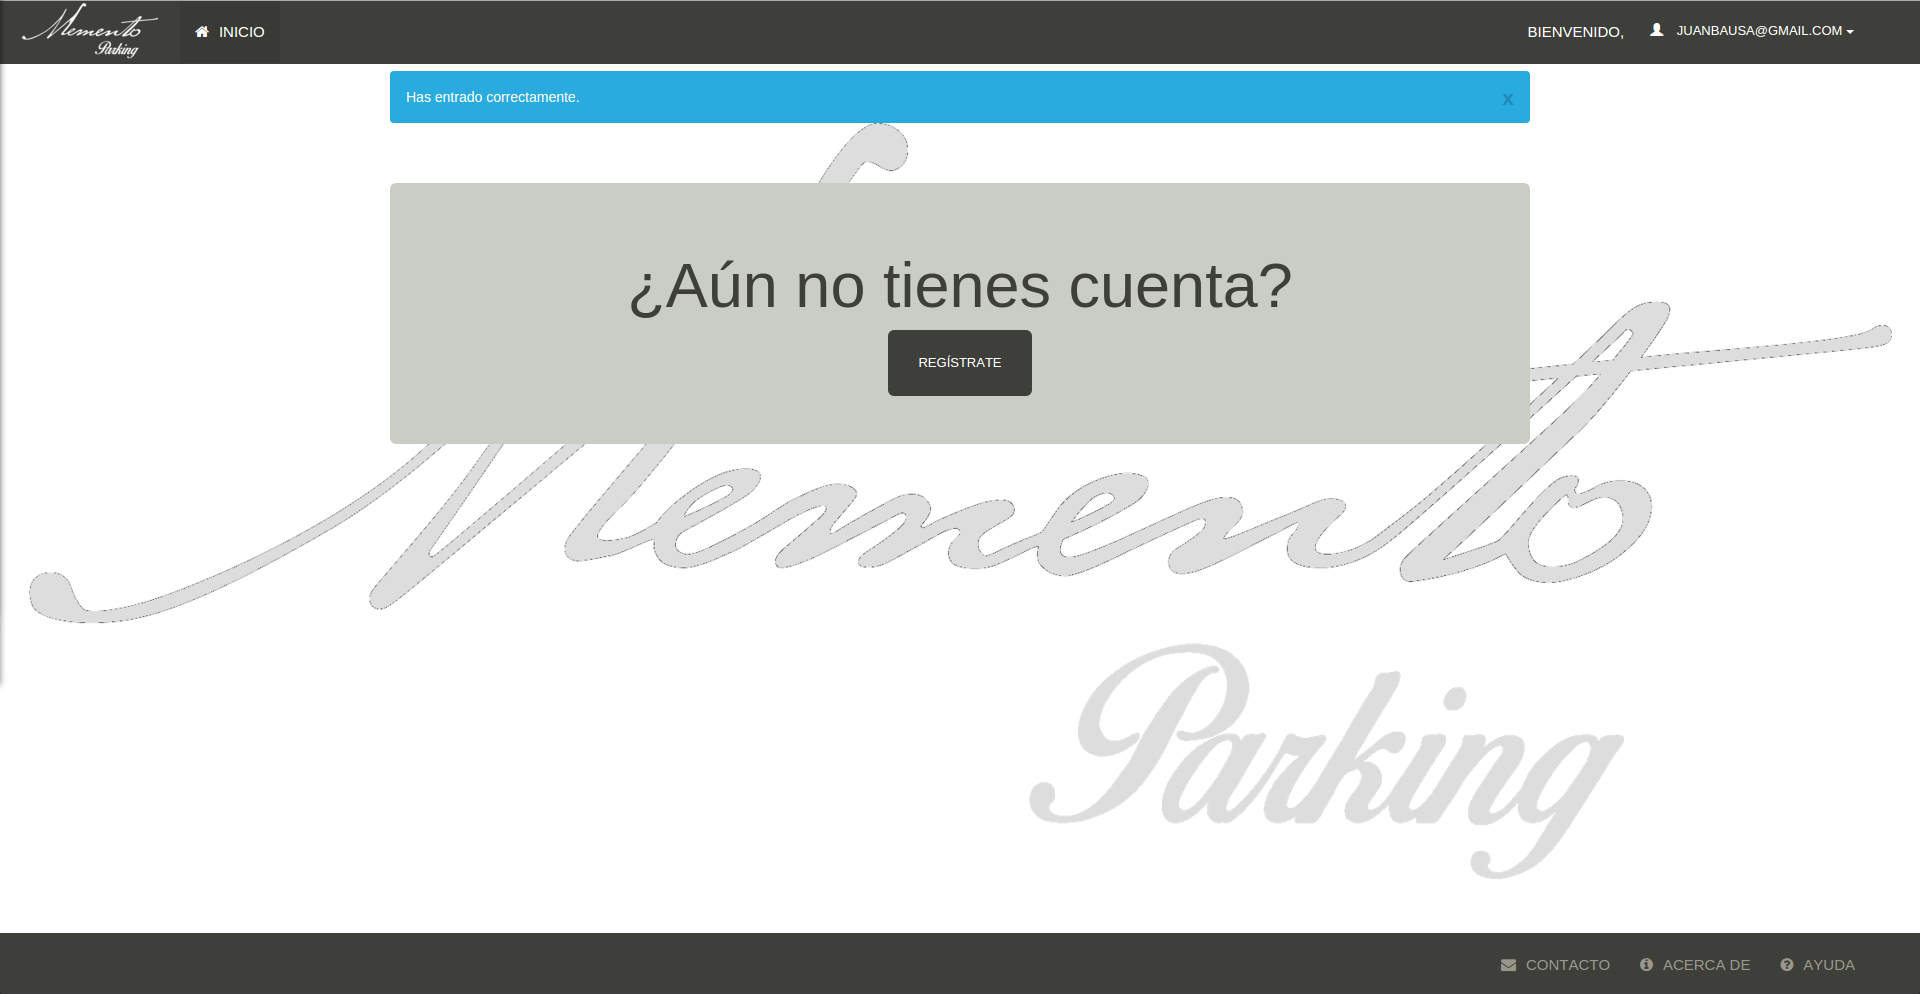
\includegraphics[width=15cm, fbox={\fboxrule} 4mm]{images/06-manual/04-home_sign_in.png}
		\caption{Página inicio autenticado}
		\label{fig:home_sign_in}
	\end{figure}

Pulsando en el menú de la esquina superior derecha tendremos acceso a las distintas herramientas que nos ofrece el sistema (ver figura \ref{fig:lateral-menu}). Seleccionando la opción de \textit{MIS DATOS} accederemos a un formulario que nos permitirá modificar algunos datos básicos de nuestro usuario (ver figura \ref{fig:edit-user}), pudiendo introducir nuestro nombre y apellidos, permitiendo que cambiemos nuestra contraseña de acceso o eliminando completamente nuestra cuenta si así lo deseamos. Para confirmar los cambios es necesario introducir la contraseña actual del usuario y pulsar en el botón \textit{CONFIRMAR CAMBIOS}.

	\begin{figure}[h!]
		\centering
		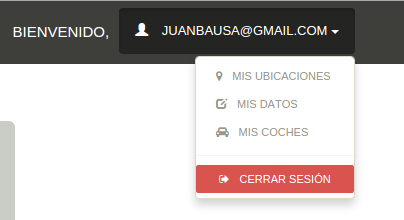
\includegraphics[width=15cm, fbox={\fboxrule} 4mm]{images/06-manual/05-lateral_menu.png}
		\caption{Menú usuario}
		\label{fig:lateral-menu}
	\end{figure}

	\begin{figure}[h!]
		\centering
		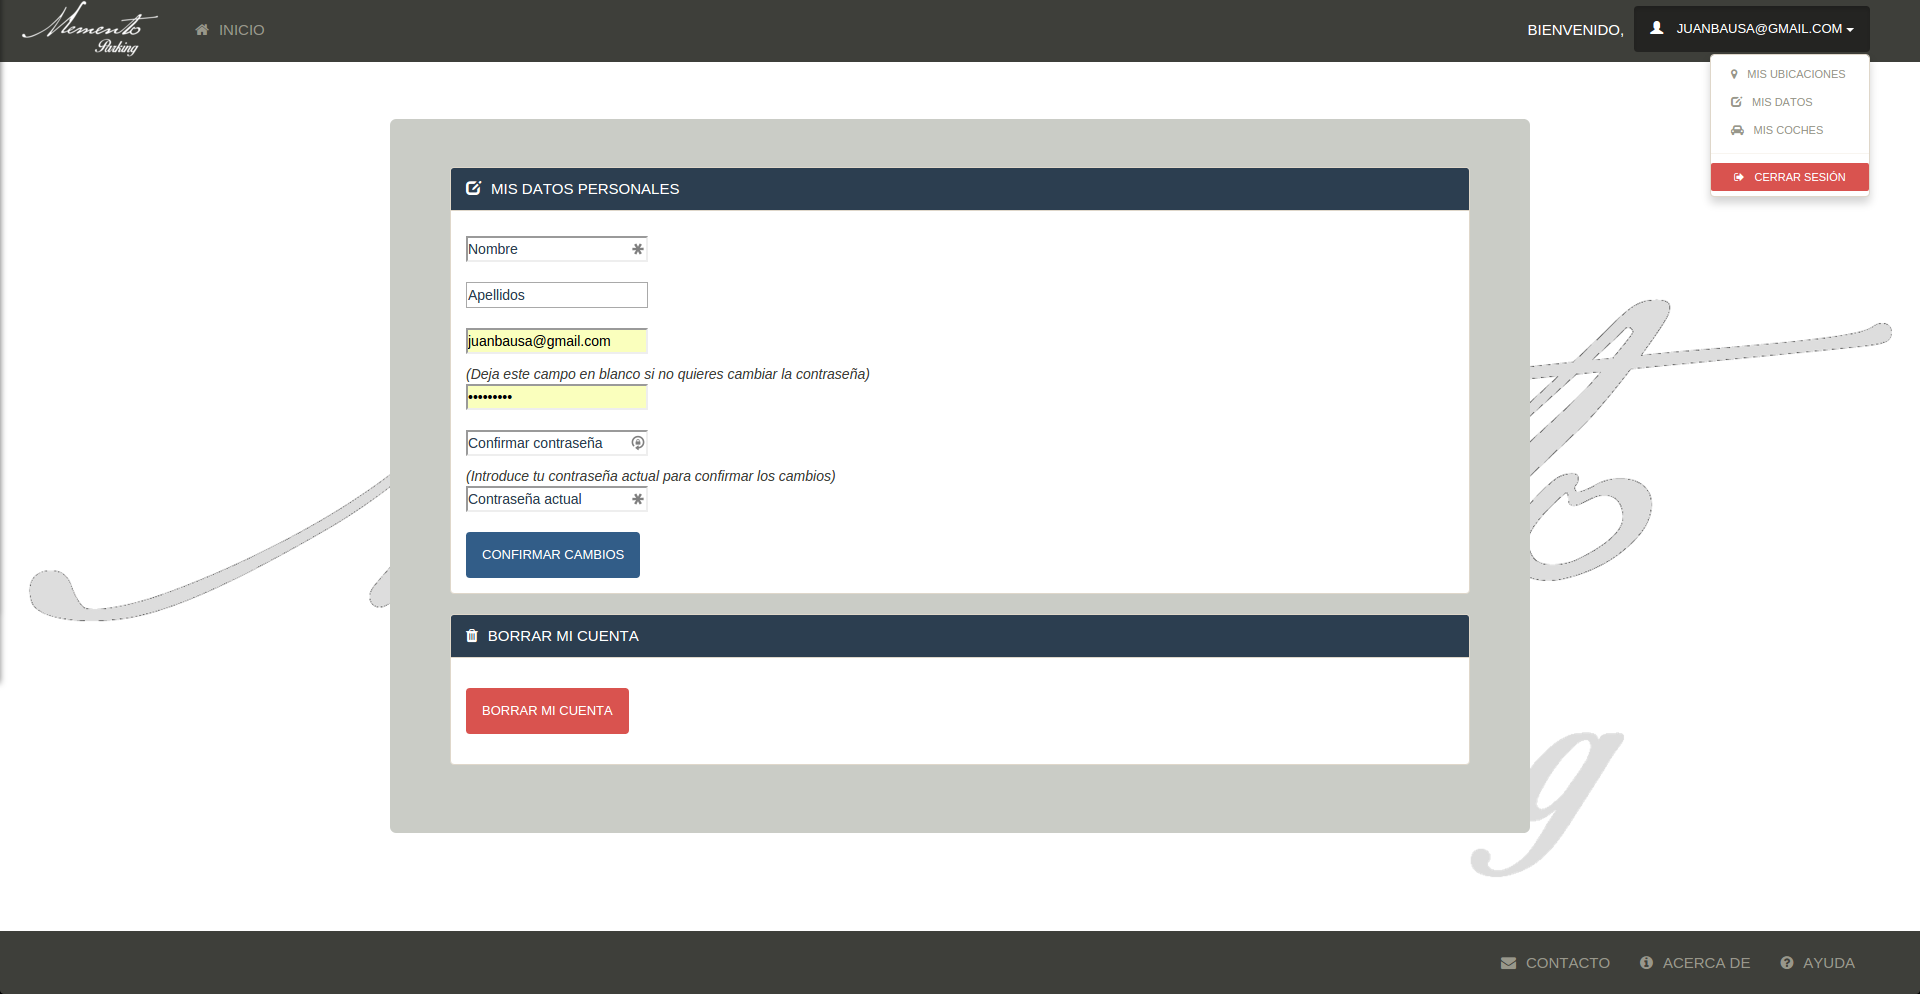
\includegraphics[width=15cm, fbox={\fboxrule} 4mm]{images/06-manual/06-edit_user.png}
		\caption{Edición usuario}
		\label{fig:edit-user}
	\end{figure}

Accediendo a la opción de \textit{MIS COCHES} podemos crear nuevos coches (para indicar más tarde donde lo hemos aparcado) o bien editar aquellos previamente creados. En la figura \ref{fig:my-car} se observa como el usuario tiene dos coches creados (Toyotita y Azulito). Seleccionando uno de estos dos coches podemos modificar la descripción o permitir que otros usuarios puedan modificar su ubicación (ver figura \ref{fig:my-car2}). Para guardar los cambios basta con pulsar el botón \textit{GUARDAR CAMBIOS}. También podemos eliminar el coche con el botón homónimo y dejar de compartirlo con los usuarios que elijamos pulsando sobre el botón de cierre que existe en cada una de las etiquetas con los correos de las personas con los que estamos compartiendo el coche seleccionado (ver figura \ref{fig:my-car3}).

	\begin{figure}[h!]
		\centering
		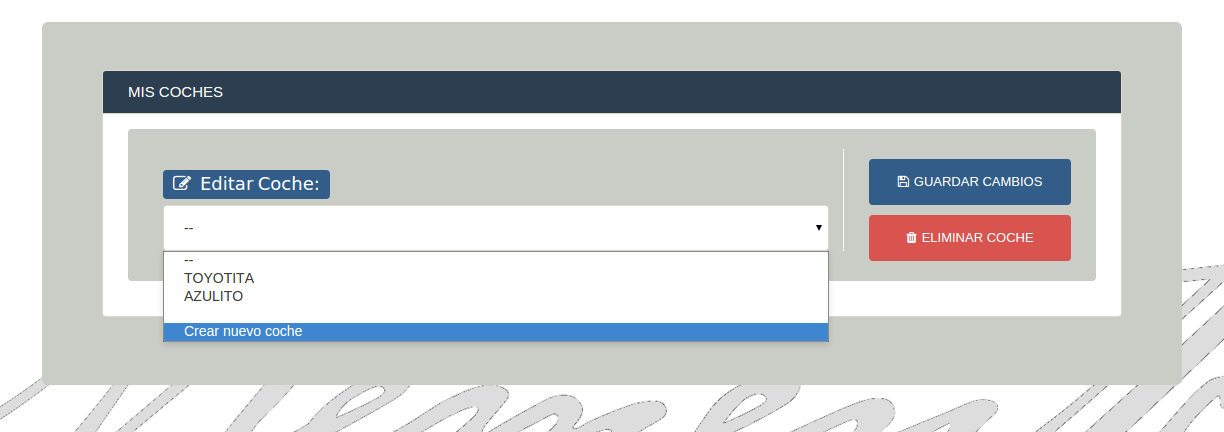
\includegraphics[width=15cm, fbox={\fboxrule} 4mm]{images/06-manual/07-my_car.png}
		\caption{Seleccionar coche}
		\label{fig:my-car}
	\end{figure}
	
	\begin{figure}[h!]
		\centering
		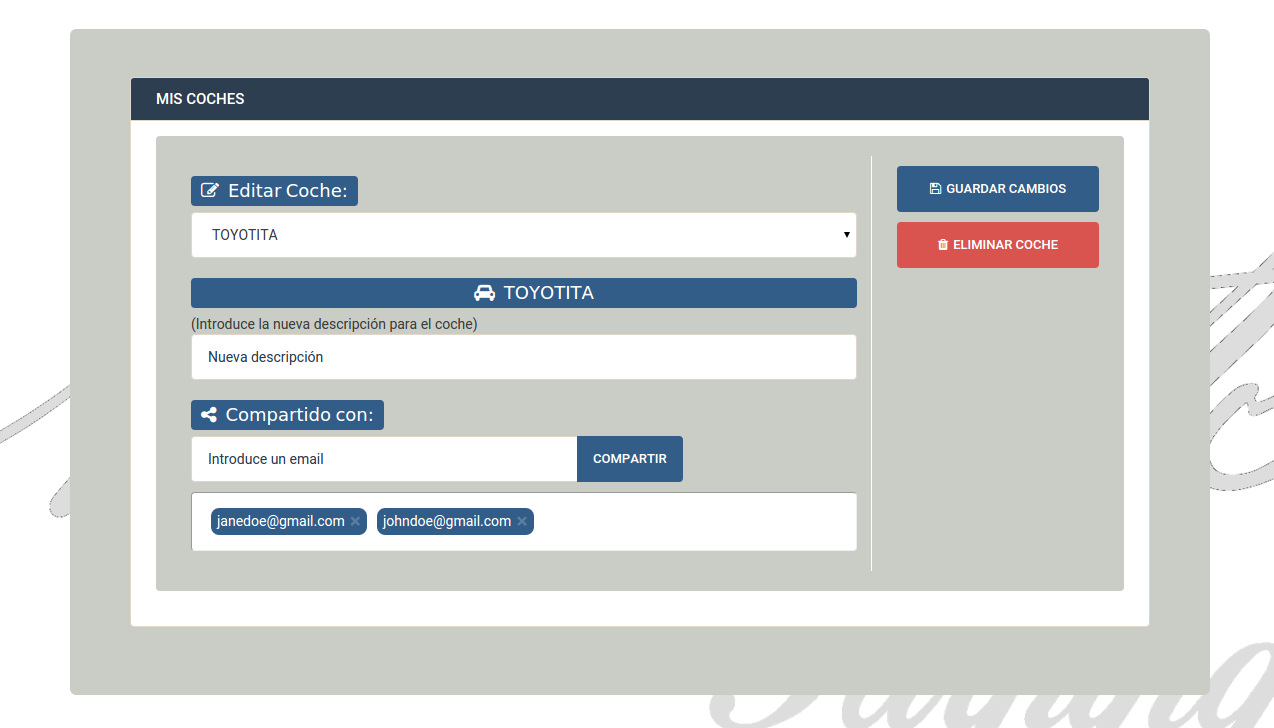
\includegraphics[width=15cm, fbox={\fboxrule} 4mm]{images/06-manual/08-my_car2.png}
		\caption{Edición coche}
		\label{fig:my-car2}
	\end{figure}

	\begin{figure}[h!]
		\centering
		
\includegraphics[width=15cm, fbox={\fboxrule} 4mm]{images/06-manual/09-my_car3.png}
		\caption{Edición usuarios compartidos}
		\label{fig:my-car3}
	\end{figure}

Pulsando en la opción \textit{MIS UBICACIONES} (ver figura \ref{fig:lateral-menu}) accedemos a la página donde se encuentra el mapa con nuestra ubicación y los marcadores de nuestros coches y los que otros usuarios han compartido con nosotros (ver figura \ref{fig:my-map}).
Debajo del mapa se encuentra el apartado \textit{MIS UBICACIONES} donde se encuentran en formato de texto las direcciones de los coches y una serie de botones para completar las distintas acciones que permite la herramienta (ver figura \ref{fig:my-map2}).

	\begin{figure}[h!]
		\centering
		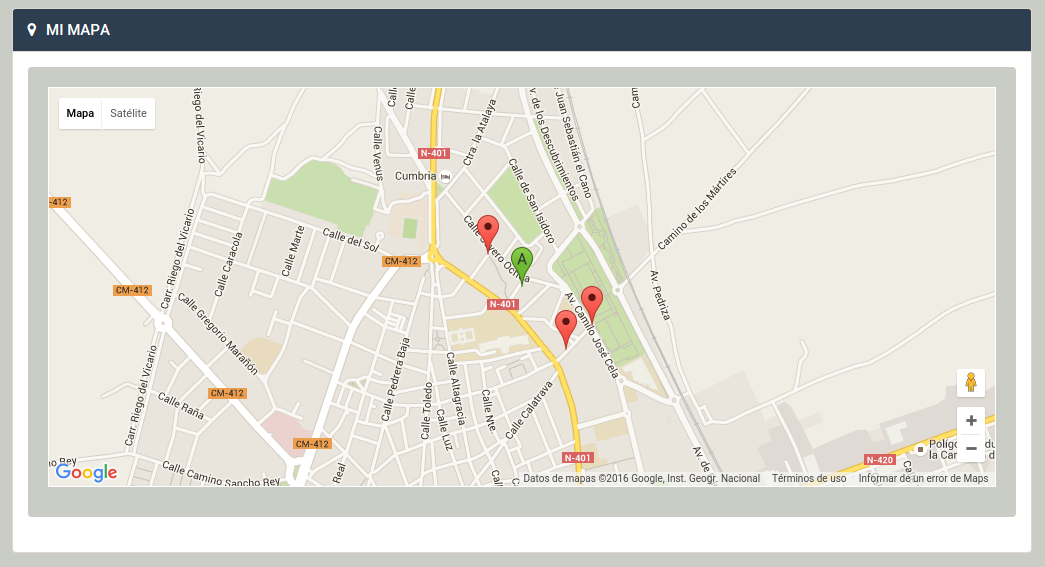
\includegraphics[width=15cm, fbox={\fboxrule} 4mm]{images/06-manual/10-my_maps.png}
		\caption{Vista previa del mapa}
		\label{fig:my-map}
	\end{figure}

	\begin{figure}[h!]
		\centering
		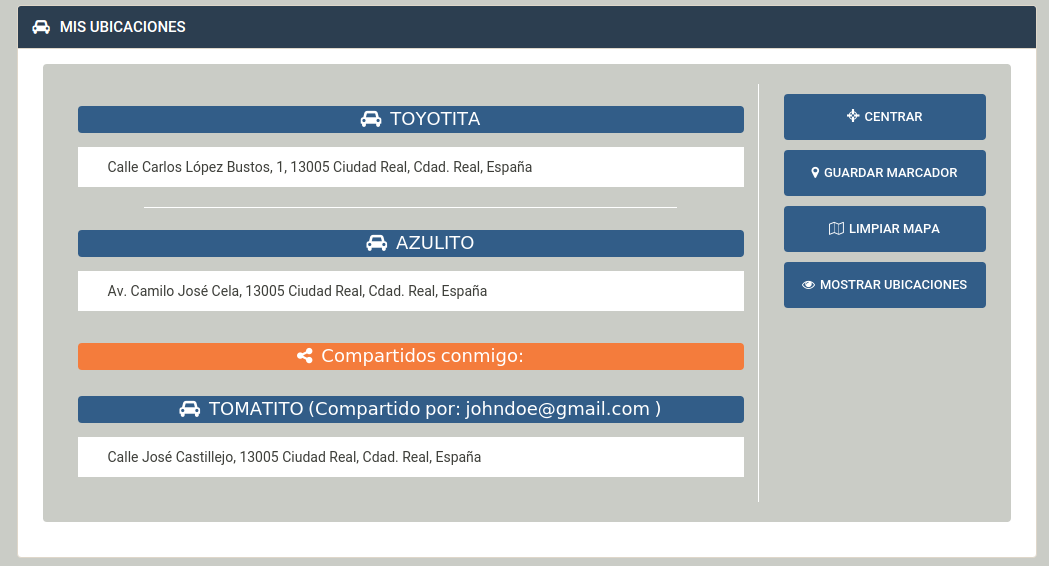
\includegraphics[width=15cm, fbox={\fboxrule} 4mm]{images/06-manual/11-my_maps2.png}
		\caption{Vista previa del apartado \textit{MIS UBICACIONES}}
		\label{fig:my-map2}
	\end{figure}
	
	El botón \textit{CENTRAR}, tal y como su nombre indica permite centrar el mapa en la posición actual del usuario, el botón \textit{GUARDAR MARCADOR} es el encargado de guardar las nuevas ubicaciones que seleccionemos, el botón \textit{LIMPIAR MAPA} hace desaparecer todos los marcadores del mapa, excepto el que indica nuestra posición actual y por último el botón \textit{MOSTRAR UBICACIONES} que se encarga de volver a mostrar todos los marcadores.
	Seleccionando un coche en este apartado, conseguiremos que solo aparezca su marcador en el mapa y que nos muestre una ruta a pie desde nuestra ubicación hasta la ubicación del coche (ver figura \ref{fig:my-map3}).
	Cuando pulsamos con el ratón encima del mapa, aparecerá un nuevo marcador de color azul indicando la posición que hemos elegido, y pulsando el botón \textit{GUARDAR MARCADOR} lograremos actualizar la posición del coche seleccionado (ver figura \ref{fig:my-map4}).

	\begin{figure}[h!]
		\centering
		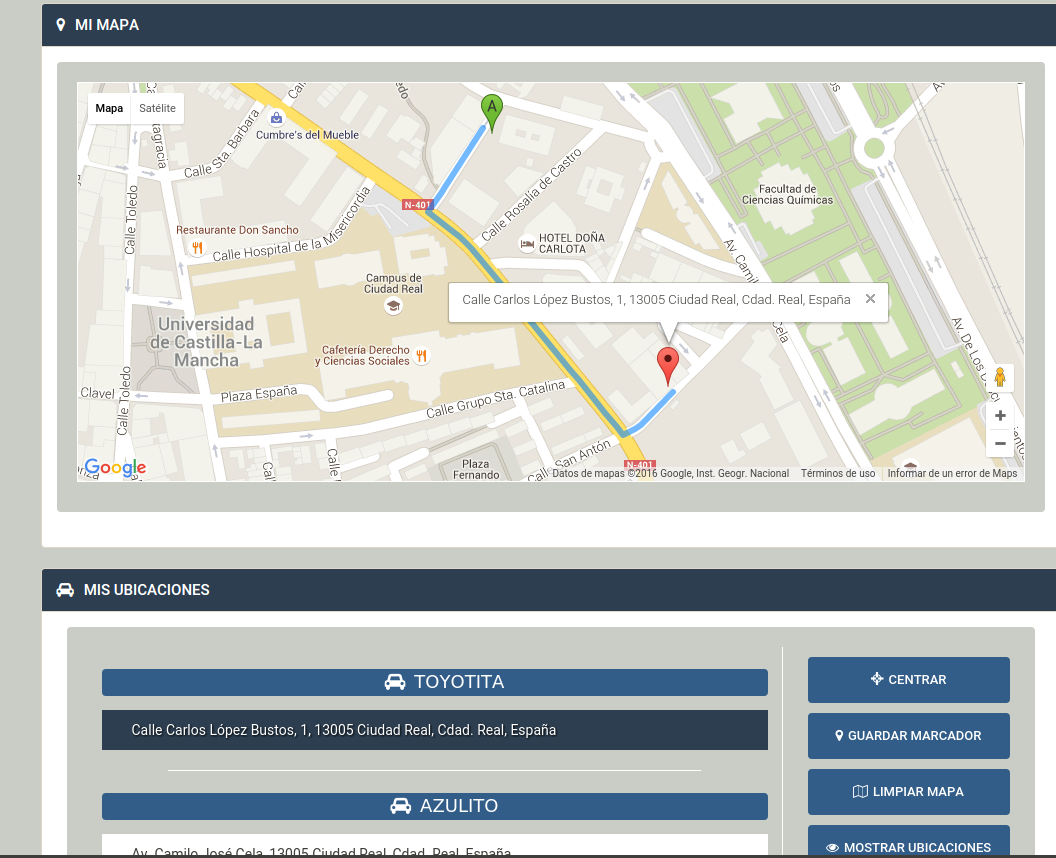
\includegraphics[width=15cm, fbox={\fboxrule} 4mm]{images/06-manual/12-my_maps3.png}
		\caption{Mapa con un coche seleccionado}
		\label{fig:my-map3}
	\end{figure}
	
	\begin{figure}[h!]
		\centering
		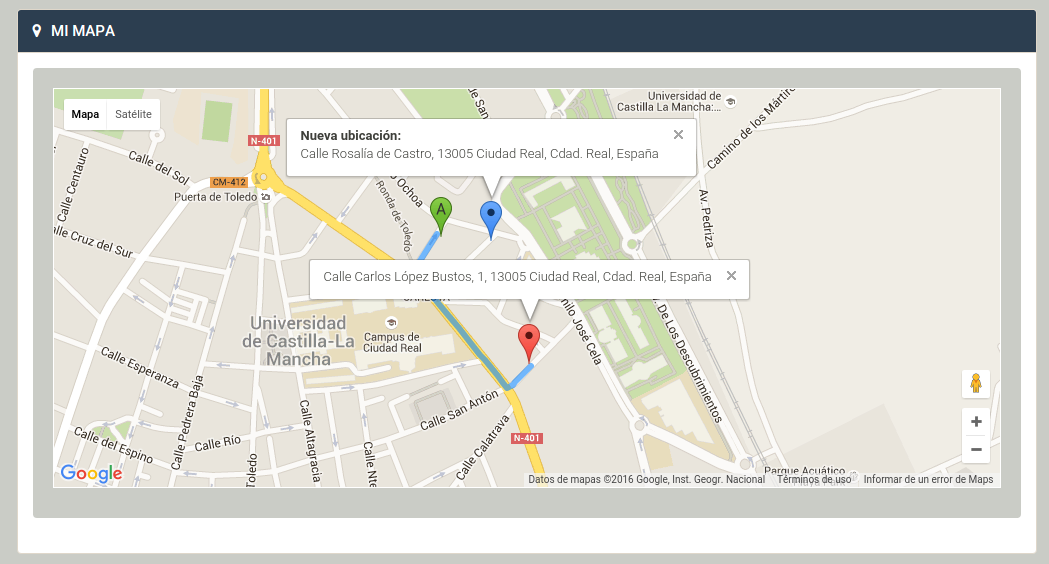
\includegraphics[width=15cm, fbox={\fboxrule} 4mm]{images/06-manual/13-my_maps4.png}
		\caption{Mapa con un coche seleccionado}
		\label{fig:my-map4}
	\end{figure}
	
	Pulsando en el botón \textit{CERRAR SESIÓN} en el menú desplegable, saldremos de nuestra cuenta y volveremos a la página de inicio.
	
% Local Variables:
%  coding: utf-8
%  mode: latex
%  mode: flyspell
%  ispell-local-dictionary: "castellano8"
% End: